\documentclass[12]{article}%12pt即为*四号字
\usepackage{ctex}%引入中文包
\usepackage{graphicx}%插入图片的包
\usepackage{geometry}%设置A4纸页边距的包
\usepackage{url}
\usepackage{stfloats}
\usepackage{float}
\usepackage{amssymb}
\usepackage{listings}
\geometry{left=3.18cm,right=3.18cm,top=2.54cm,bottom=2.54cm}%设置页边距
\linespread{1}%设置行间距


\begin{document}
\begin{center}
    \LARGE\songti\textbf{微分方程数值解Project3作业报告} \\%标题
    \large\kaishu\textbf{褚朱钇恒\qquad 3200104144}%一般是我的姓名
\end{center}
\section{运行说明}
    本项目需要调用\verb|jsoncpp|与\verb|eigen3|库,故请在运行此项目前安装好这两个包。
    
    您可以使用以下命令进行安装:

    \begin{lstlisting}
        sudo apt-get install libeigen3-dev
        sudo apt-get install libjsoncpp-dev
    \end{lstlisting}

    在\verb|project|目录下使用\verb|make|命令即可编译运行整个项目并得到实验报告。

    如果您只需要渲染文档,可以使用\verb|make report|命令

\section{程序设计思路}
    设计了\verb|IVPsolver|基类,用于求解微分方程,它派生了两个类
    \begin{itemize}
        \item LMM:线性多步法
        \item RKM:龙格库塔法
    \end{itemize}

    前者派生了三个类,分别实现了\verb|AdamsBashforth|,\verb|AdamsMoulton|,\verb|BackDifferFormula|法;三者支持

    后者派生了五个类,分别实现了\verb|classicalRK|,\verb|DormandPrinceRK|,
    \verb|ESDIRK|,\verb|FehlbergRK|,\verb|GaussLegendreRK|法;
    其中\verb|DormandPrinceRK_solver|实现了自适应步长。

    此外,本程序还实现了classFactory方便调用各类求解器,由于constuctor 属性是GNU C编译器的一个扩展,不是标准的C语言特性,为了更好的移植性,没有使用该参数。

\section{数值求解结果}
\subsection{第一部分}
对于(11.199)$k=[0.004,0.002,0.001,0.0005]$的结果(图为k=0.0005的结果)如下(为了避免迭代无法控制精度导致死循环,ESDIRK的步长为其他的$\frac{1}{10}$
\begin{figure}[H]
    \centering
    \begin{minipage}[t]{0.3\textwidth}
    \centering
    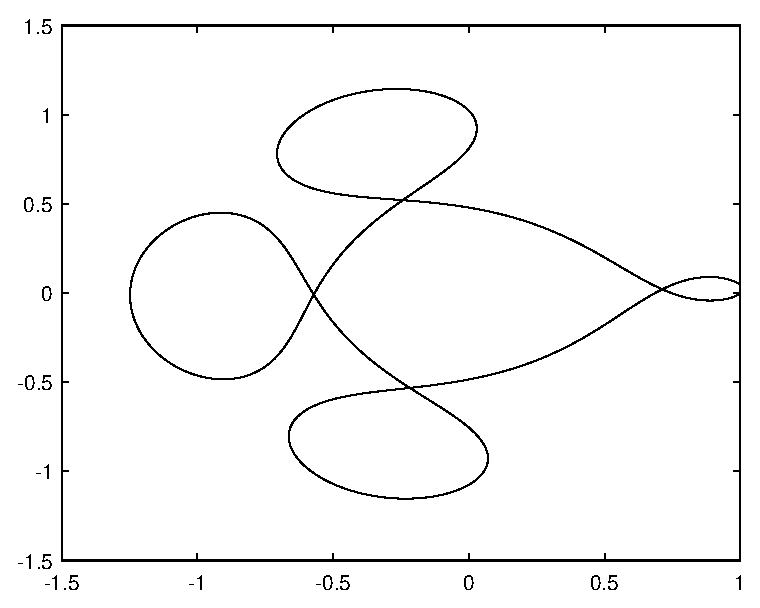
\includegraphics[width=4cm]{../pic/ABF1.eps}
    \caption{ABF}
    \end{minipage}
    \begin{minipage}[t]{0.3\textwidth}
    \centering
    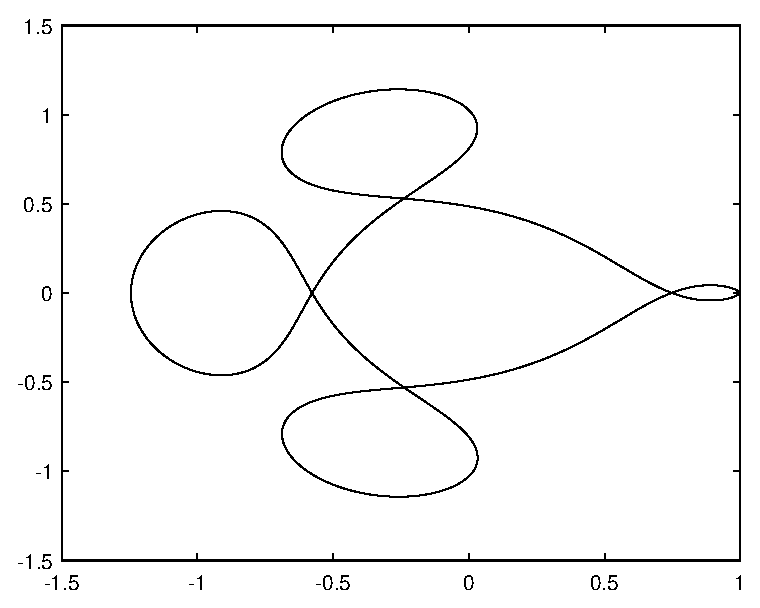
\includegraphics[width=4cm]{../pic/ADM1.eps}
    \caption{ADM}
    \end{minipage}
    \begin{minipage}[t]{0.3\textwidth}
    \centering
    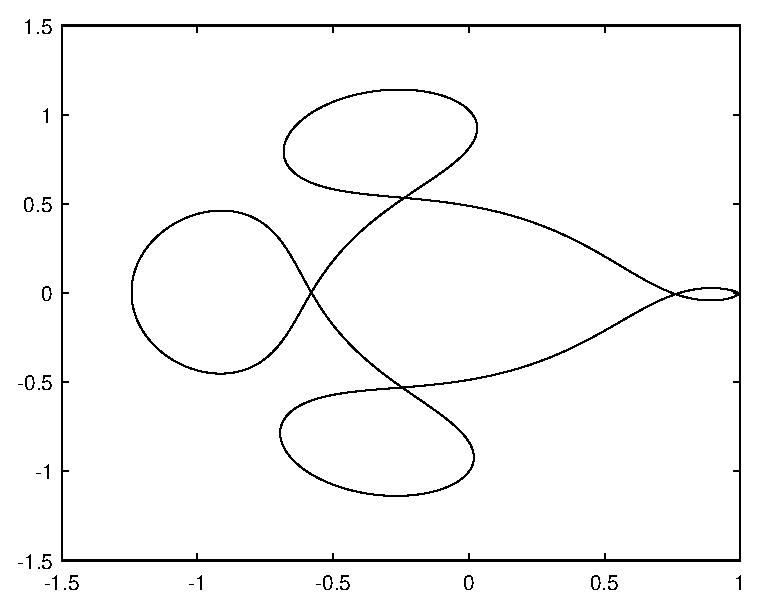
\includegraphics[width=4cm]{../pic/BDF1.eps}
    \caption{BDM}
    \end{minipage}
\end{figure}
\begin{figure}[H]
    \centering
    \begin{minipage}[t]{0.3\textwidth}
    \centering
    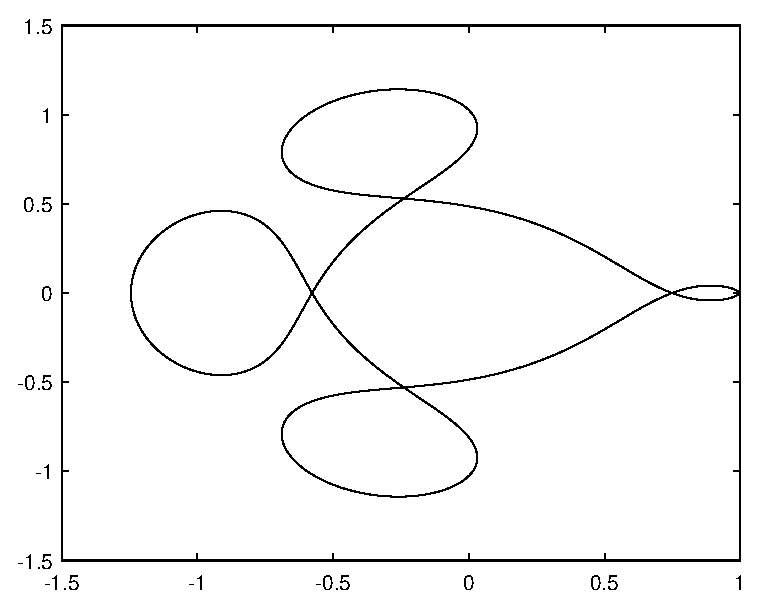
\includegraphics[width=4cm]{../pic/RK1.eps}
    \caption{classicalRK}
    \end{minipage}
    \begin{minipage}[t]{0.3\textwidth}
    \centering
    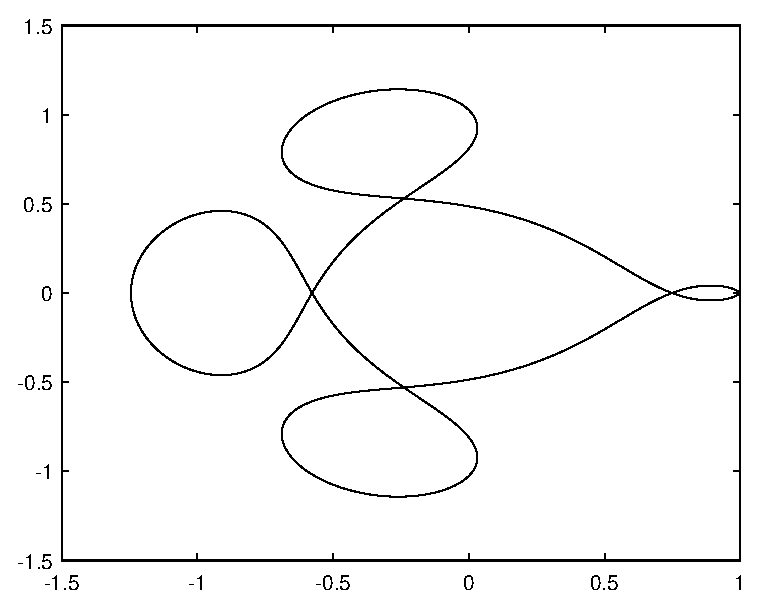
\includegraphics[width=4cm]{../pic/DormandPrinceRK1.eps}
    \caption{Dormand-Prince}
    \end{minipage}
    \begin{minipage}[t]{0.3\textwidth}
    \centering
    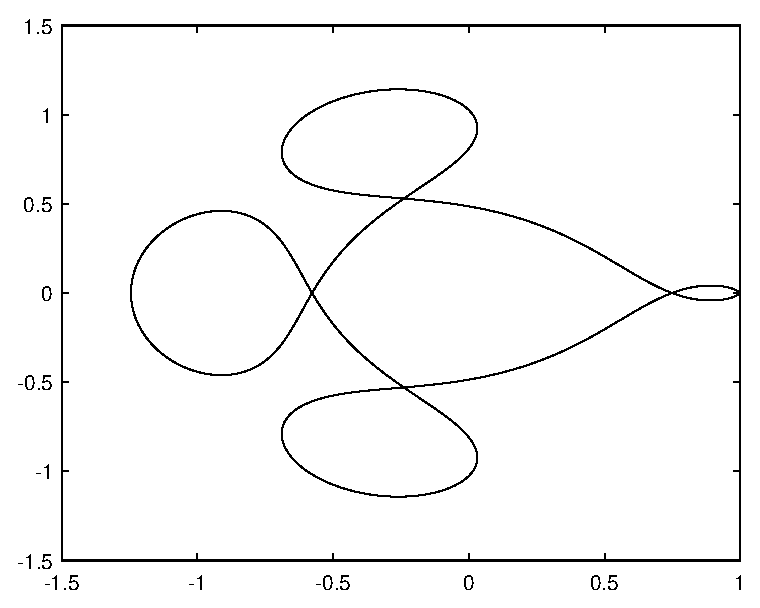
\includegraphics[width=4cm]{../pic/ESDIRK1.eps}
    \caption{ESDIRK}
    \end{minipage}
\end{figure}
\begin{figure}[H]
    \centering
    \begin{minipage}[t]{0.48\textwidth}
    \centering
    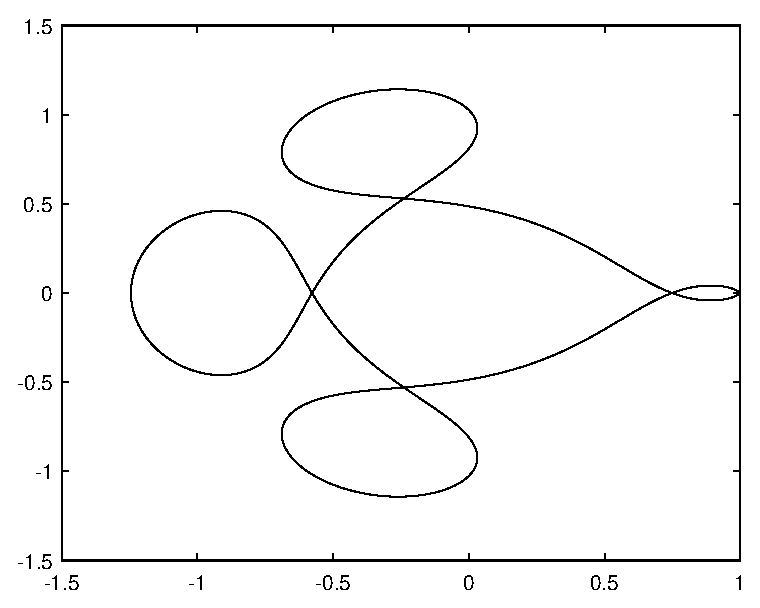
\includegraphics[width=5cm]{../pic/FehlbergRK1.eps}
    \caption{FehlbergRK}
    \end{minipage}
    \begin{minipage}[t]{0.48\textwidth}
    \centering
    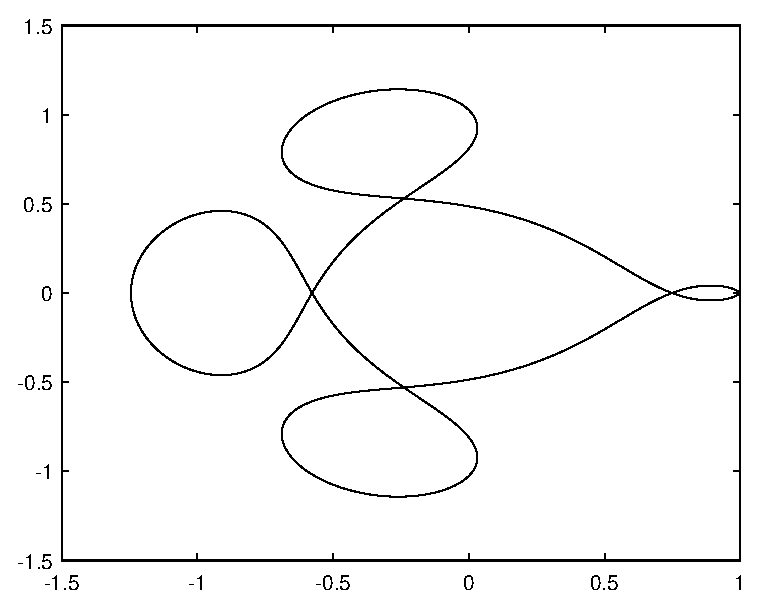
\includegraphics[width=5cm]{../pic/GaussLegendreRK1.eps}
    \caption{GaussLegendreRK}
    \end{minipage}
\end{figure}
收敛速度和运算时间的详细信息在data文件夹中,由于测试组数过多,此处仅给出几个例子并画出图像。

\begin{figure}[H]
    \centering
    \begin{minipage}[t]{0.48\textwidth}
    \centering
    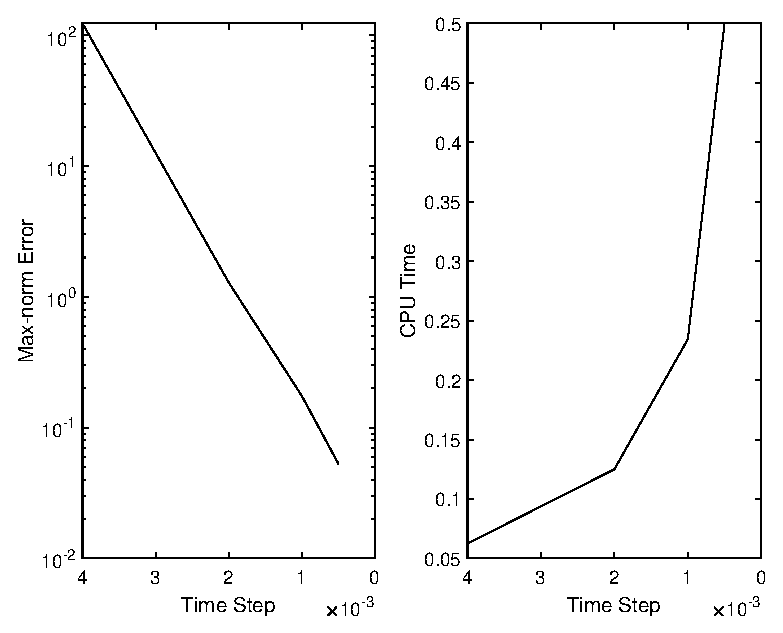
\includegraphics[width=6cm]{../pic/AdamsBashforth4test1.eps}
    \caption{AdamsBashforth p=4}
    \end{minipage}
    \begin{minipage}[t]{0.48\textwidth}
    \centering
    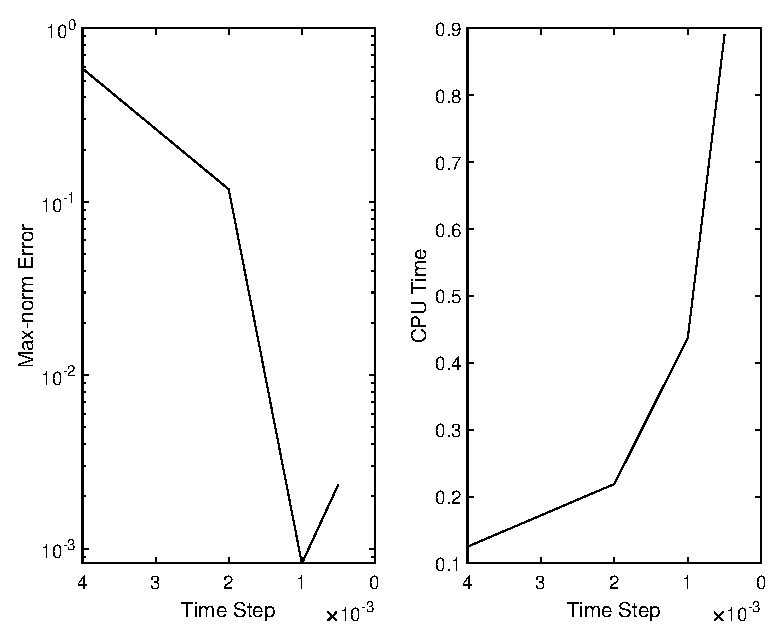
\includegraphics[width=6cm]{../pic/AdamsMoulton5test1.eps}
    \caption{ADM p=5}
    \end{minipage}
\end{figure}
\begin{figure}[H]
    \centering
    \begin{minipage}[t]{0.48\textwidth}
    \centering
    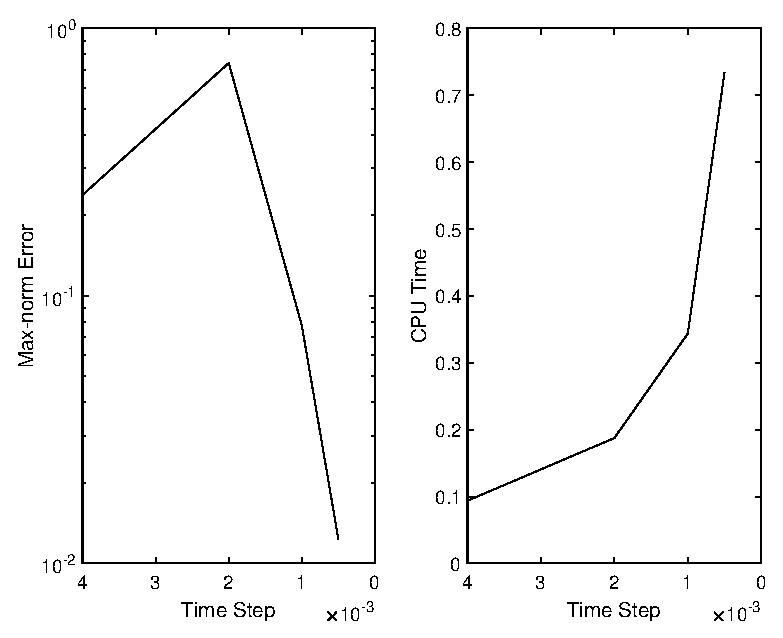
\includegraphics[width=6cm]{../pic/BackDifferFormula4test1.eps}
    \caption{BDM p=4}
    \end{minipage}
    \begin{minipage}[t]{0.48\textwidth}
    \centering
    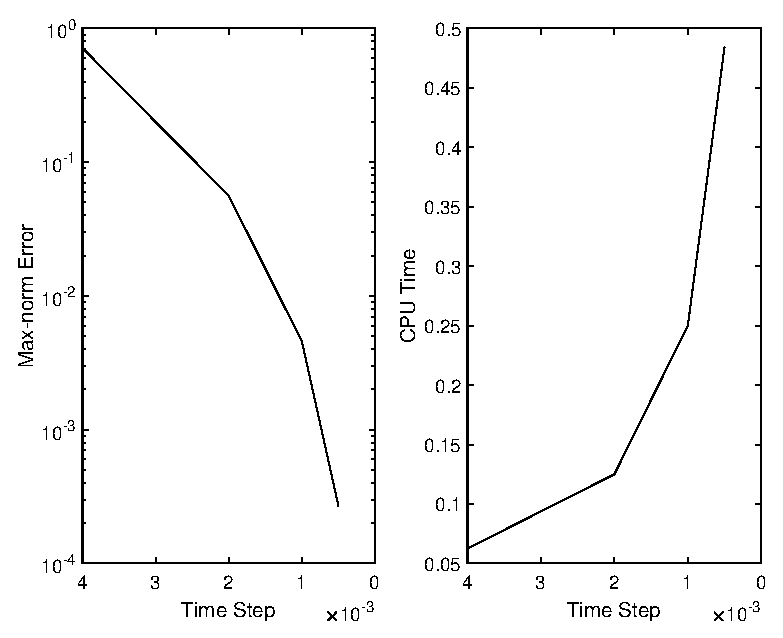
\includegraphics[width=6cm]{../pic/classicalRK4test1.eps}
    \caption{classicalRK}
    \end{minipage}
\end{figure}
\begin{figure}[H]
    \centering
    \begin{minipage}[t]{0.48\textwidth}
    \centering
    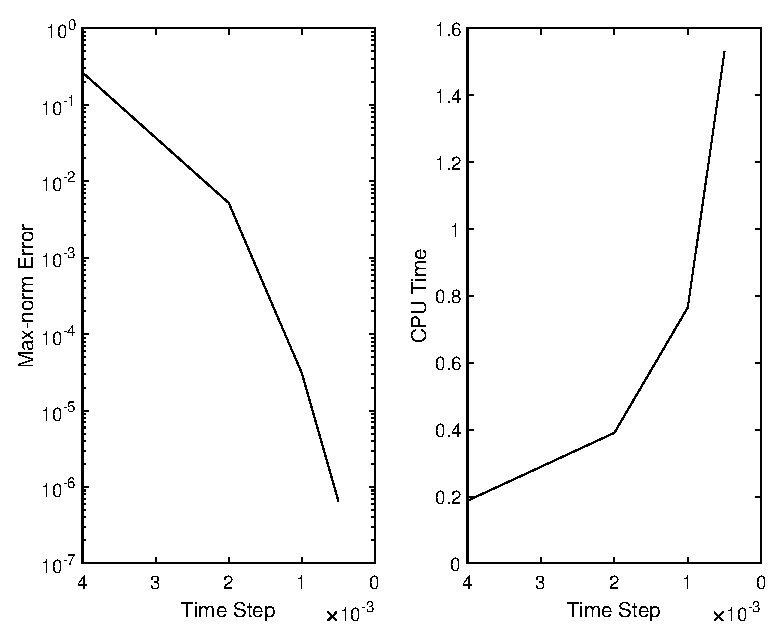
\includegraphics[width=6cm]{../pic/DormandPrinceRK5test1.eps}
    \caption{Dormand-Prince p=5}
    \end{minipage}
    \begin{minipage}[t]{0.48\textwidth}
    \centering
    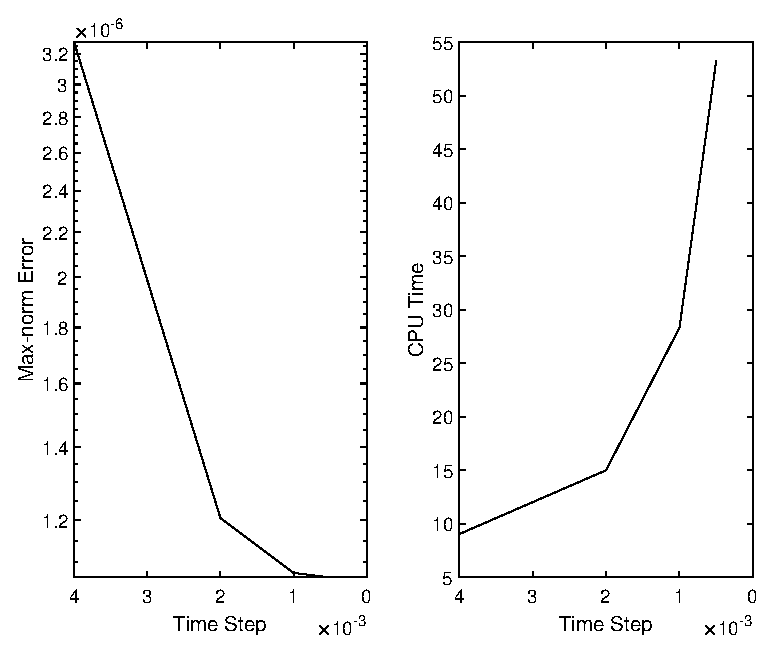
\includegraphics[width=6cm]{../pic/ESDIRK5test1.eps}
    \caption{ESDIRK}
    \end{minipage}
\end{figure}
\begin{figure}[H]
    \centering
    \begin{minipage}[t]{0.48\textwidth}
    \centering
    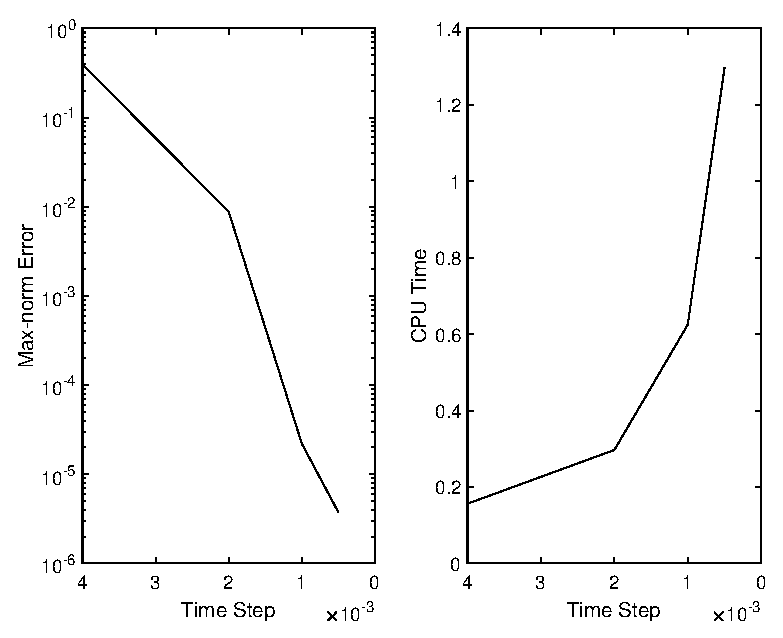
\includegraphics[width=6cm]{../pic/FehlbergRK5test1.eps}
    \caption{FehlbergRK p=5}
    \end{minipage}
    \begin{minipage}[t]{0.48\textwidth}
    \centering
    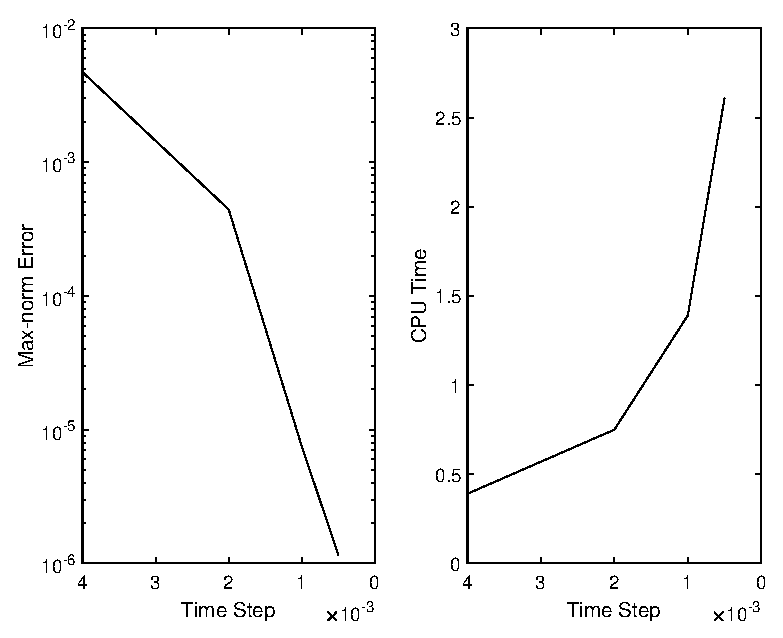
\includegraphics[width=6cm]{../pic/GaussLegendreRK3test1.eps}
    \caption{GaussLegendreRK p=3}
    \end{minipage}
\end{figure}


对于(11.200)$k=[0.004,0.002,0.001,0.0005]$的结果(图为k=0.0005的结果)(为了避免迭代无法控制精度导致死循环,ESDIRK的步长为其他的$\frac{1}{10}$
\begin{figure}[H]
    \centering
    \begin{minipage}[t]{0.3\textwidth}
    \centering
    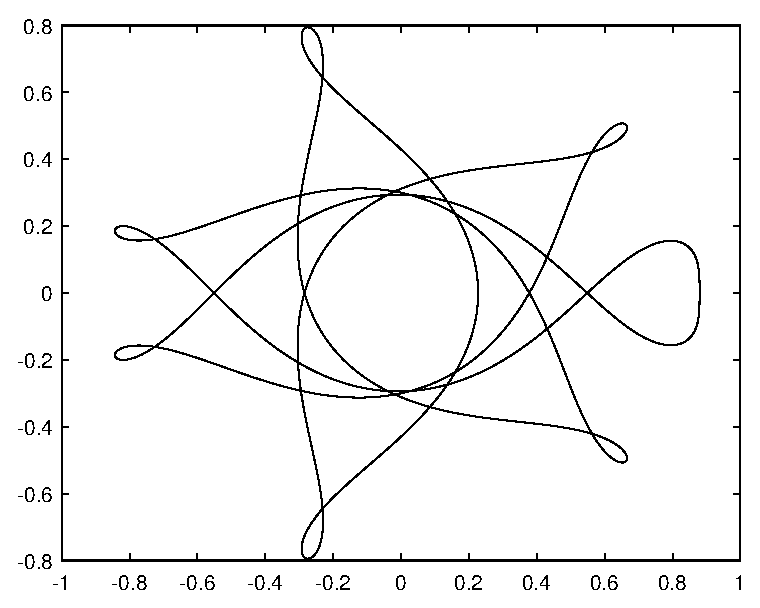
\includegraphics[width=4cm]{../pic/ABF.eps}
    \caption{ABF}
    \end{minipage}
    \begin{minipage}[t]{0.3\textwidth}
    \centering
    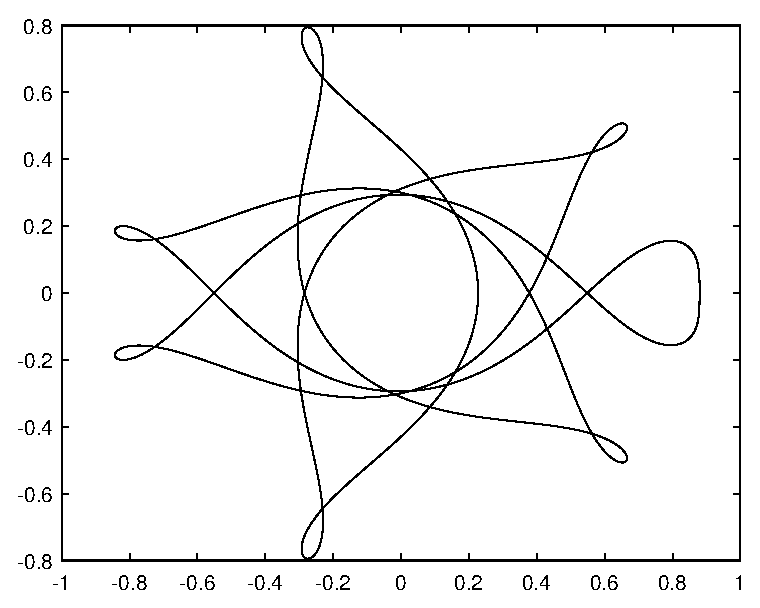
\includegraphics[width=4cm]{../pic/ADM.eps}
    \caption{ADM}
    \end{minipage}
    \begin{minipage}[t]{0.3\textwidth}
    \centering
    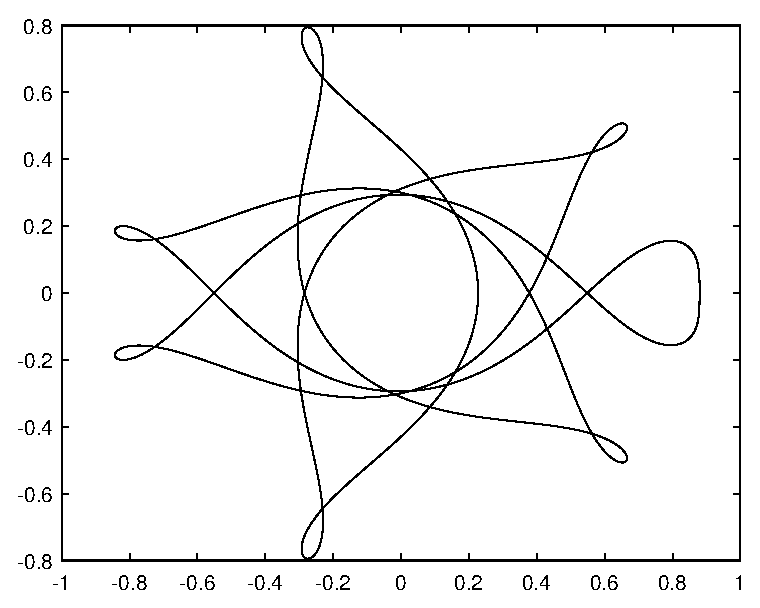
\includegraphics[width=4cm]{../pic/BDF.eps}
    \caption{BDM}
    \end{minipage}
\end{figure}
\begin{figure}[H]
    \centering
    \begin{minipage}[t]{0.3\textwidth}
    \centering
    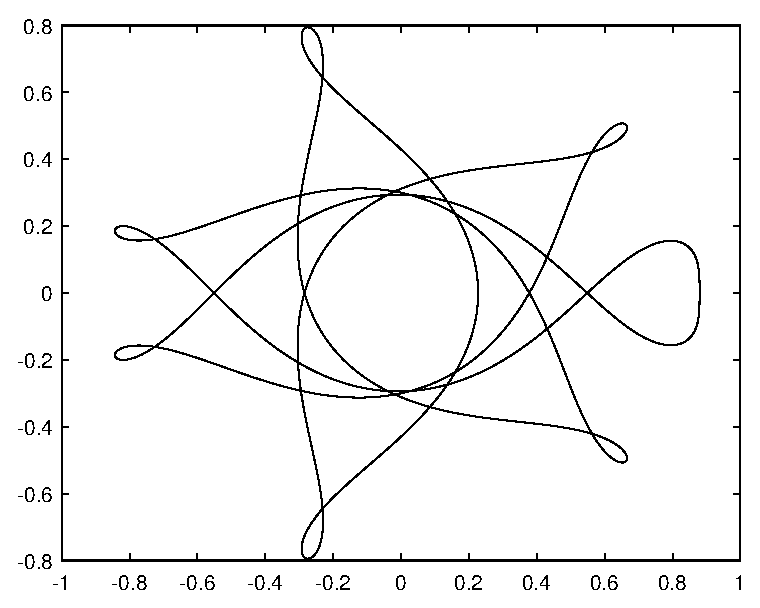
\includegraphics[width=4cm]{../pic/RK.eps}
    \caption{classicalRK}
    \end{minipage}
    \begin{minipage}[t]{0.3\textwidth}
    \centering
    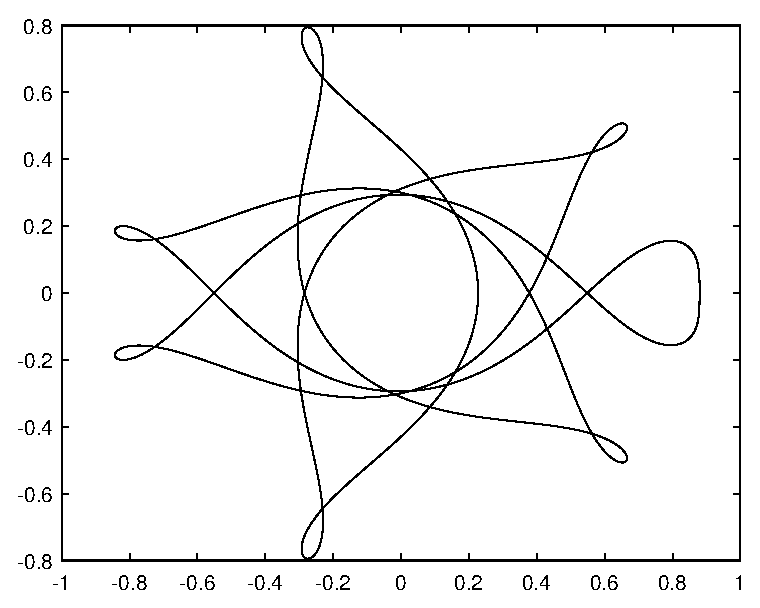
\includegraphics[width=4cm]{../pic/DormandPrinceRK.eps}
    \caption{Dormand-Prince}
    \end{minipage}
    \begin{minipage}[t]{0.3\textwidth}
    \centering
    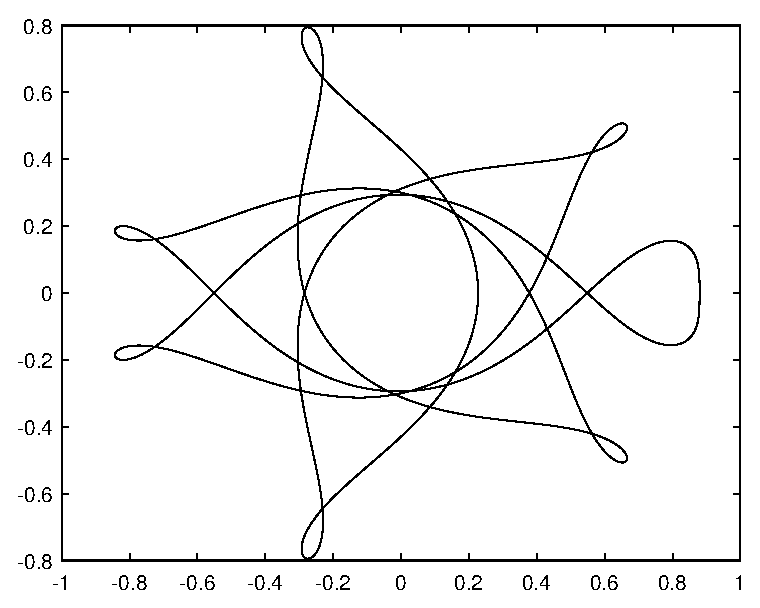
\includegraphics[width=4cm]{../pic/ESDIRK.eps}
    \caption{ESDIRK}
    \end{minipage}
\end{figure}
\begin{figure}[H]
    \centering
    \begin{minipage}[t]{0.48\textwidth}
    \centering
    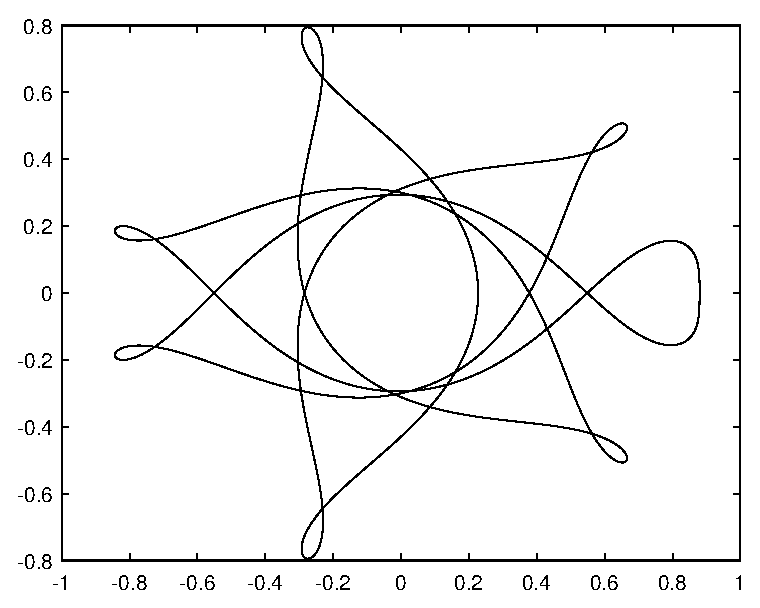
\includegraphics[width=5cm]{../pic/FehlbergRK.eps}
    \caption{FehlbergRK}
    \end{minipage}
    \begin{minipage}[t]{0.48\textwidth}
    \centering
    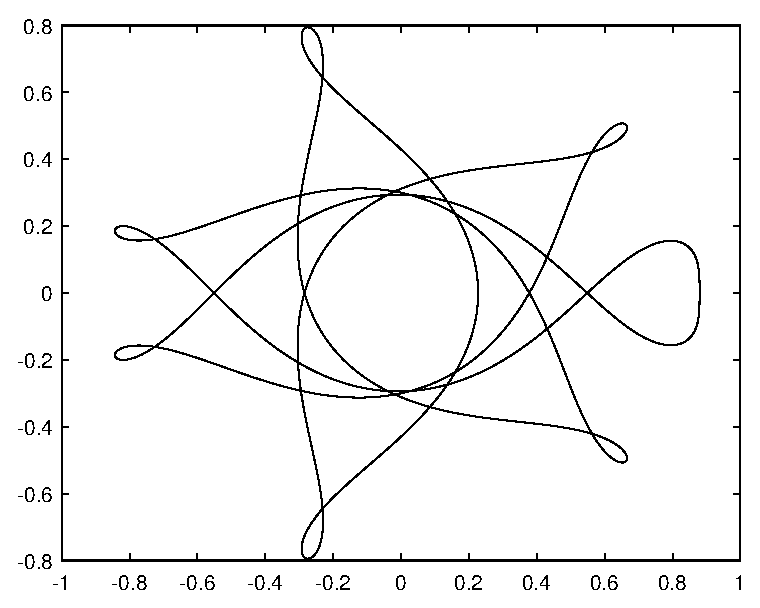
\includegraphics[width=5cm]{../pic/GaussLegendreRK.eps}
    \caption{GaussLegendreRK}
    \end{minipage}
\end{figure}

收敛速度和运算时间的详细信息在data文件夹中,由于测试组数过多,此处仅给出几个例子并画出图像。

\begin{figure}[H]
    \centering
    \begin{minipage}[t]{0.48\textwidth}
    \centering
    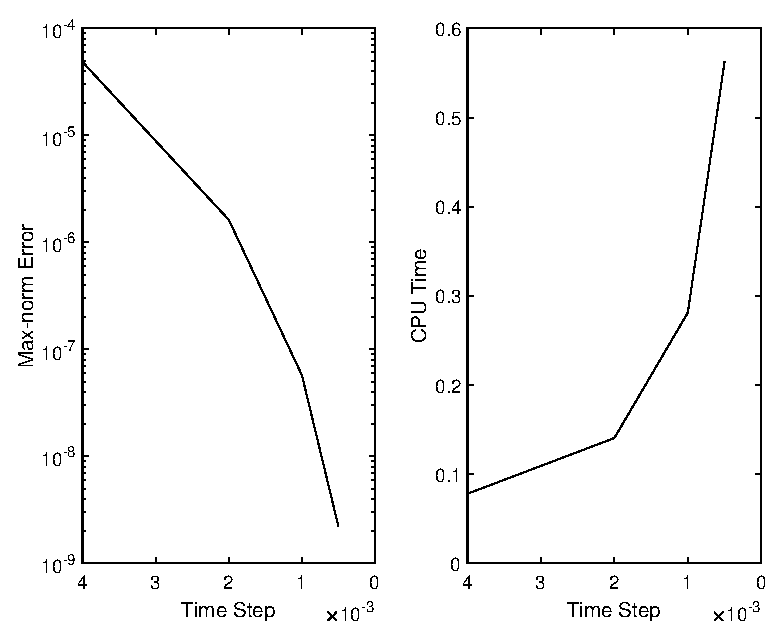
\includegraphics[width=6cm]{../pic/AdamsBashforth4test2.eps}
    \caption{AdamsBashforth p=4}
    \end{minipage}
    \begin{minipage}[t]{0.48\textwidth}
    \centering
    \includegraphics[width=6cm]{../pic/AdamsMoulton5test2.eps}
    \caption{ADM p=5}
    \end{minipage}
\end{figure}
\begin{figure}[H]
    \centering
    \begin{minipage}[t]{0.48\textwidth}
    \centering
    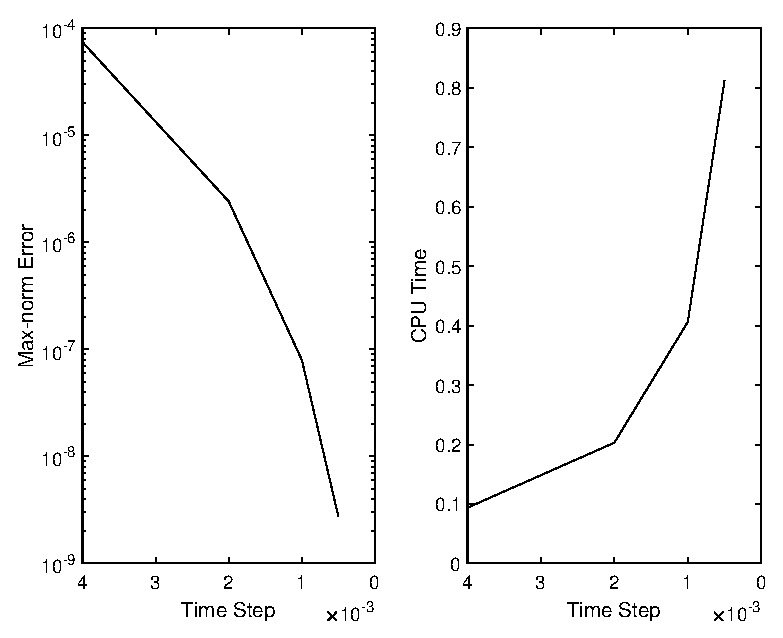
\includegraphics[width=6cm]{../pic/BackDifferFormula4test2.eps}
    \caption{BDM p=4}
    \end{minipage}
    \begin{minipage}[t]{0.48\textwidth}
    \centering
    \includegraphics[width=6cm]{../pic/classicalRK4test2.eps}
    \caption{classicalRK}
    \end{minipage}
\end{figure}
\begin{figure}[H]
    \centering
    \begin{minipage}[t]{0.48\textwidth}
    \centering
    \includegraphics[width=6cm]{../pic/DormandPrinceRK5test2.eps}
    \caption{Dormand-Prince p=5}
    \end{minipage}
    \begin{minipage}[t]{0.48\textwidth}
    \centering
    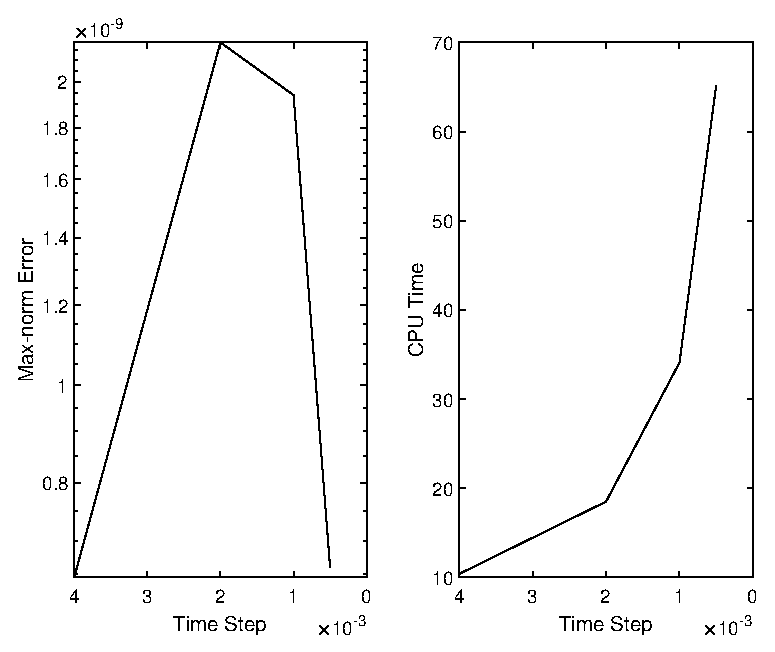
\includegraphics[width=6cm]{../pic/ESDIRK5test2.eps}
    \caption{ESDIRK}
    \end{minipage}
\end{figure}
\begin{figure}[H]
    \centering
    \begin{minipage}[t]{0.48\textwidth}
    \centering
    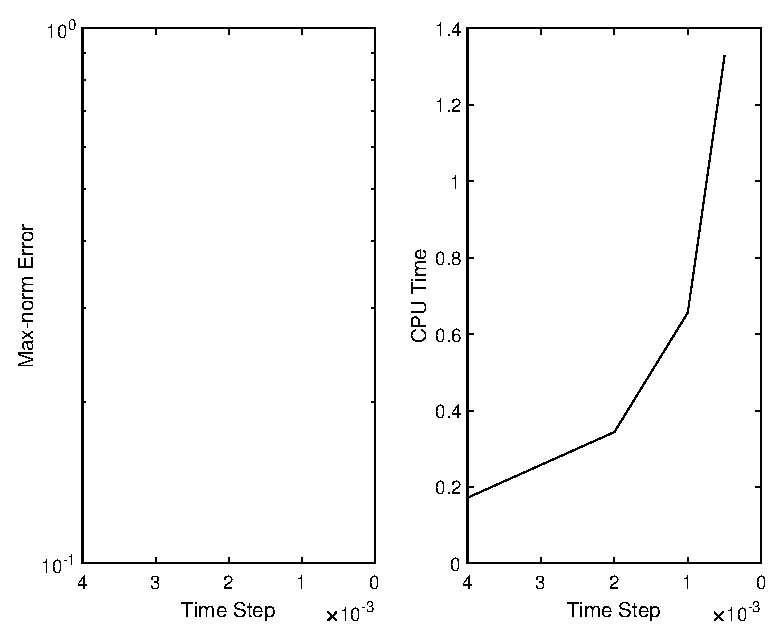
\includegraphics[width=6cm]{../pic/FehlbergRK5test2.eps}
    \caption{FehlbergRK p=5}
    \end{minipage}
    \begin{minipage}[t]{0.48\textwidth}
    \centering
    \includegraphics[width=6cm]{../pic/GaussLegendreRK3test2.eps}
    \caption{GaussLegendreRK p=3}
    \end{minipage}
\end{figure}

计算得到8个方案的收敛率分别为:
\begin{itemize}
    \item AdamsBashforth p=4: 4.7322
    \item ADM p=5: 4.7399
    \item BDM p=4: 4.9354
    \item classicalRK: 3.6432
    \item Dormand-Prince p=5: 5.0006
    \item ESDIRK: 0.8044
    \item FehlbergRK p=5: 4.7885
    \item GaussLegendreRK p=3: 4.6520
\end{itemize}

发现ESDIRK的收敛阶似乎于理论不符,查询数据发现由于为了避免迭代死循环,步长减小了10倍,而此时的误差已达到$10^{-6}$接近设置的$eps=10^{-9}$,小于其他方法的误差,所以可能是浮点误差导致的问题。
此外,某些方法在某条轨道上误差可能不太收敛,可能是机器精度的问题,此处挑选了更符合理论的一条。

\subsection{第二部分}
测试 Euler 方法 24000 步,经典 RK 方法 6000 步,Dormand-Prince 方法使用自动控制步长 100 步,图像如下:

\begin{figure}[H]
    \centering
    \begin{minipage}[t]{0.3\textwidth}
    \centering
    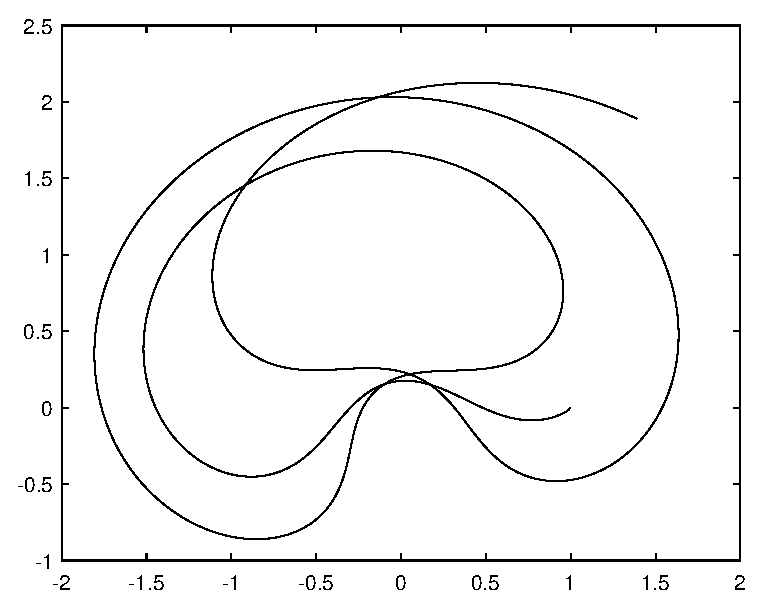
\includegraphics[width=4cm]{../pic/Euler.eps}
    \caption{Euler}
    \end{minipage}
    \begin{minipage}[t]{0.3\textwidth}
    \centering
    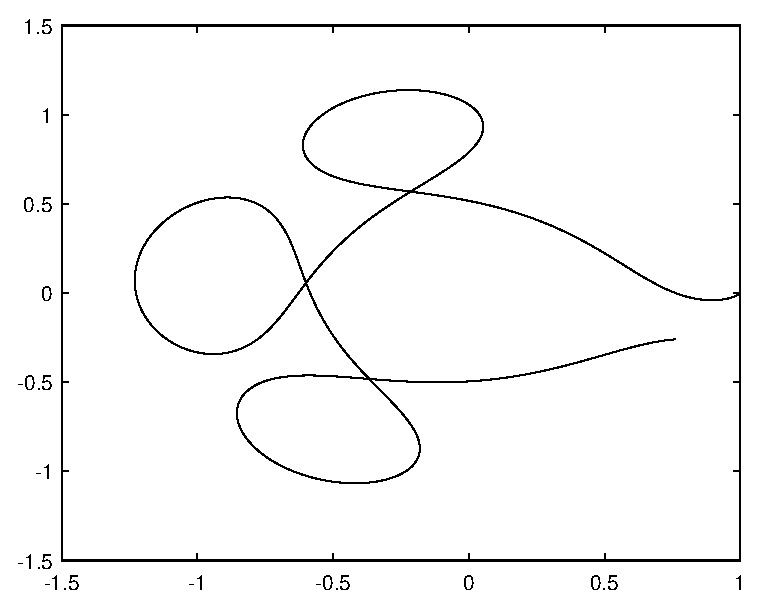
\includegraphics[width=4cm]{../pic/RK6000.eps}
    \caption{ClassicalRK}
    \end{minipage}
    \begin{minipage}[t]{0.3\textwidth}
    \centering
    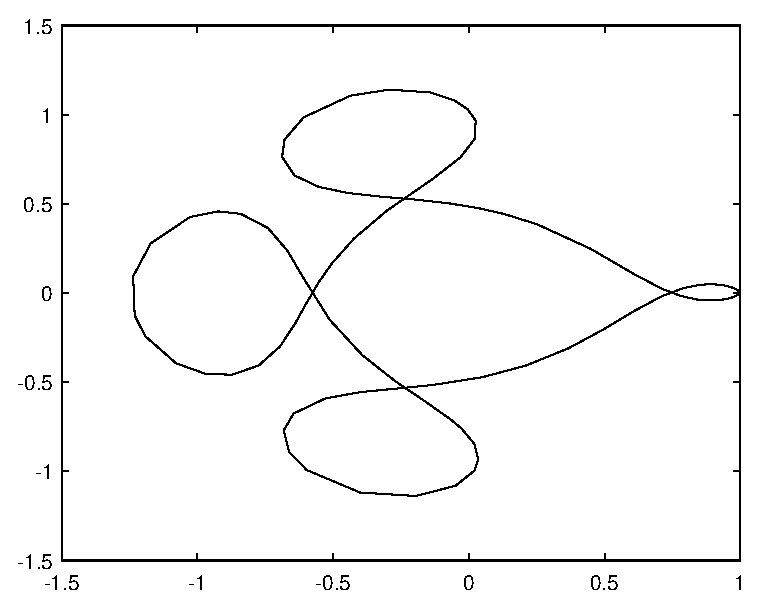
\includegraphics[width=4cm]{../pic/Dormand-Prince.eps}
    \caption{Dormand-Prince }
    \end{minipage}
\end{figure}

经测试发现,步长从 k = 0.004 开始减小,Euler 方法最快,直至k=0.0005都不能达到精度要求;经典 RK 方法在
k = 0.0005 时达到精度要求,用时为0.484375s;Dormand-Prince 方法在
k = 0.001 时达到精度要求,用时为0.765625s。

所以如果仅考虑步长和精度的关系,经典 RK 方法胜利;如果仅考虑时间和精度的关系,Dormand-Prince 方法胜利,

具体数据可见data文件夹下的AdamsBashforth1test1,classicalRK4test1,DormandPrinceRK5test1.
\end{document} 